\section{Fold}

In the general case, functions of two parameters are \textbf{not associative}, so the order in which one carries out the \textbf{combination of the elements matters}. On lists, there are two obvious ways to carry this out: either by recursively combining the first element with the results of combining the rest (called a right fold) or by recursively combining the results of combining all but the last element with the last one, (called a left fold). 

\begin{lstlisting}[language=Haskell]
-- f :: a -> a -> a -> a
-- [a1, a2, a3, a4]
-- Right fold: f a1 (f a2 (f a3 a4))
-- Left fold: f (f (f a1 a2) a3) a4
\end{lstlisting}

Also, in practice, it is convenient and natural to have an initial value which in the case of a right fold, is used when one reaches the end of the list, and in the case of a left fold, is what is initially combined with the first element of the list.

\subsection{What fold does to lists}
One can view a fold on lists as replacing the nil at the end of the list with a specific value, and replacing each cons with a specific function. These replacements can be viewed as a diagram: 

\begin{center}
  \textbf{Foldr} \\
  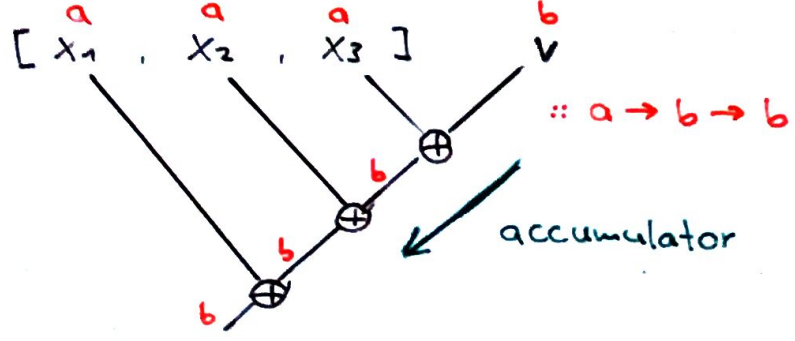
\includegraphics[width=0.6\textwidth]{figures/foldr-overview.png}
\end{center}

\begin{center}
  \textbf{Foldl} \\
  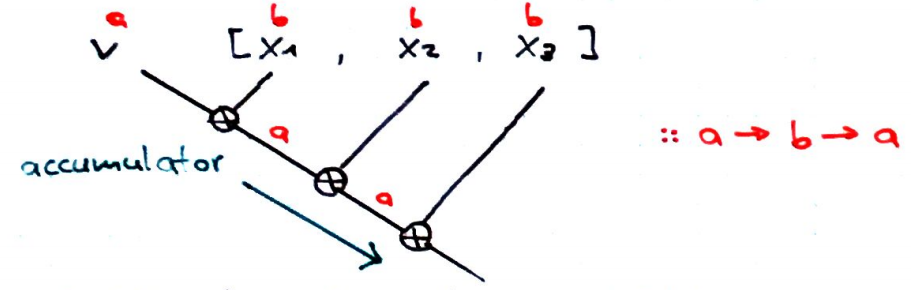
\includegraphics[width=0.7\textwidth]{figures/foldl.png}
\end{center}

They also highlight the fact that foldr (:) [] is the identity function on lists (a shallow copy in Lisp parlance), as replacing cons with cons and nil with nil will not change the result. The left fold diagram suggests an easy way to reverse a list, foldl (flip (:)) []

\clearpage
\subsection{Linear Foldr}
\begin{lstlisting}[language=Haskell]
-- if the list is empty, the result is the initial value z; else
-- apply f to the first element and the result of folding the rest

foldr' :: (a -> b -> b) -> b -> [a] -> b
foldr' f z []     = z 
foldr' f z (x:xs) = f x (foldr' f z xs) 

-- foldr' f id [a1, a2, a3, a4]
-- f a1 (foldr' f id [a2, a3, a4])
-- f a1 (f a2 (foldr' f id [a3, a4]))
-- f a1 (f a2 (f a3 (foldr' f id [a4])))
-- f a1 (f a2 (f a3 (f a4 (foldr' f id [])))
-- f a1 (f a2 (f a3 (f a4 id))
\end{lstlisting}

\subsection{Linear Foldl}

Again, the first argument to foldl should be a function that is all about taking a default value, the first element of the list, and then returning a new default for the process to continue with a shortened list.

\begin{lstlisting}[language=Haskell]
-- if the list is empty, the result is the initial value; else
-- we recurse immediately, making the new initial value the result
-- of combining the old initial value with the first element.

foldl' :: (b -> a -> b) -> b -> [a] -> b
foldl' f z []     = z                  
foldl' f z (x:xs) = foldl' f (f z x) xs

-- foldl' f id [a1, a2, a3, a4]
-- foldl' f (f id a1) [a2, a3, a4]
-- foldl' f (f (f id a1) a2) [a3, a4]
-- foldl' f (f (f (f id a1) a2) a3) [a4]
-- foldl' f (f (f (f (f id a1) a2) a3) a4) []
-- foldl' f (f (f (f (f id a1) a2) a3) a4)
-- f (f (f (f (f id a1) a2) a3) a4)
\end{lstlisting}

\subsection{Difference between reduction and fold}
Fold takes an explicit initial value for the accumulator while reduce uses the first element of the input list as the initial accumulator value.

\subsection{Tree-like folds}
\begin{lstlisting}[language=Haskell]
foldt            :: (a -> a -> a) -> a -> [a] -> a
foldt f z []     = z
foldt f z [x]    = x                             -- aka foldt' of data-ordlist
foldt f z xs     = foldt f z (pairs f xs)
 
foldi            :: (a -> a -> a) -> a -> [a] -> a
foldi f z []     = z
foldi f z (x:xs) = f x (foldi f z (pairs f xs))  -- aka foldt of data-ordlist
 
pairs            :: (a -> a -> a) -> [a] -> [a]
pairs f (x:y:t)  = f x y : pairs f t
pairs f t        = t
\end{lstlisting}

\clearpage